\section{The Totem Platform: AI and AR in Digital Art}

\begin{figure}[!h]
    \centering
    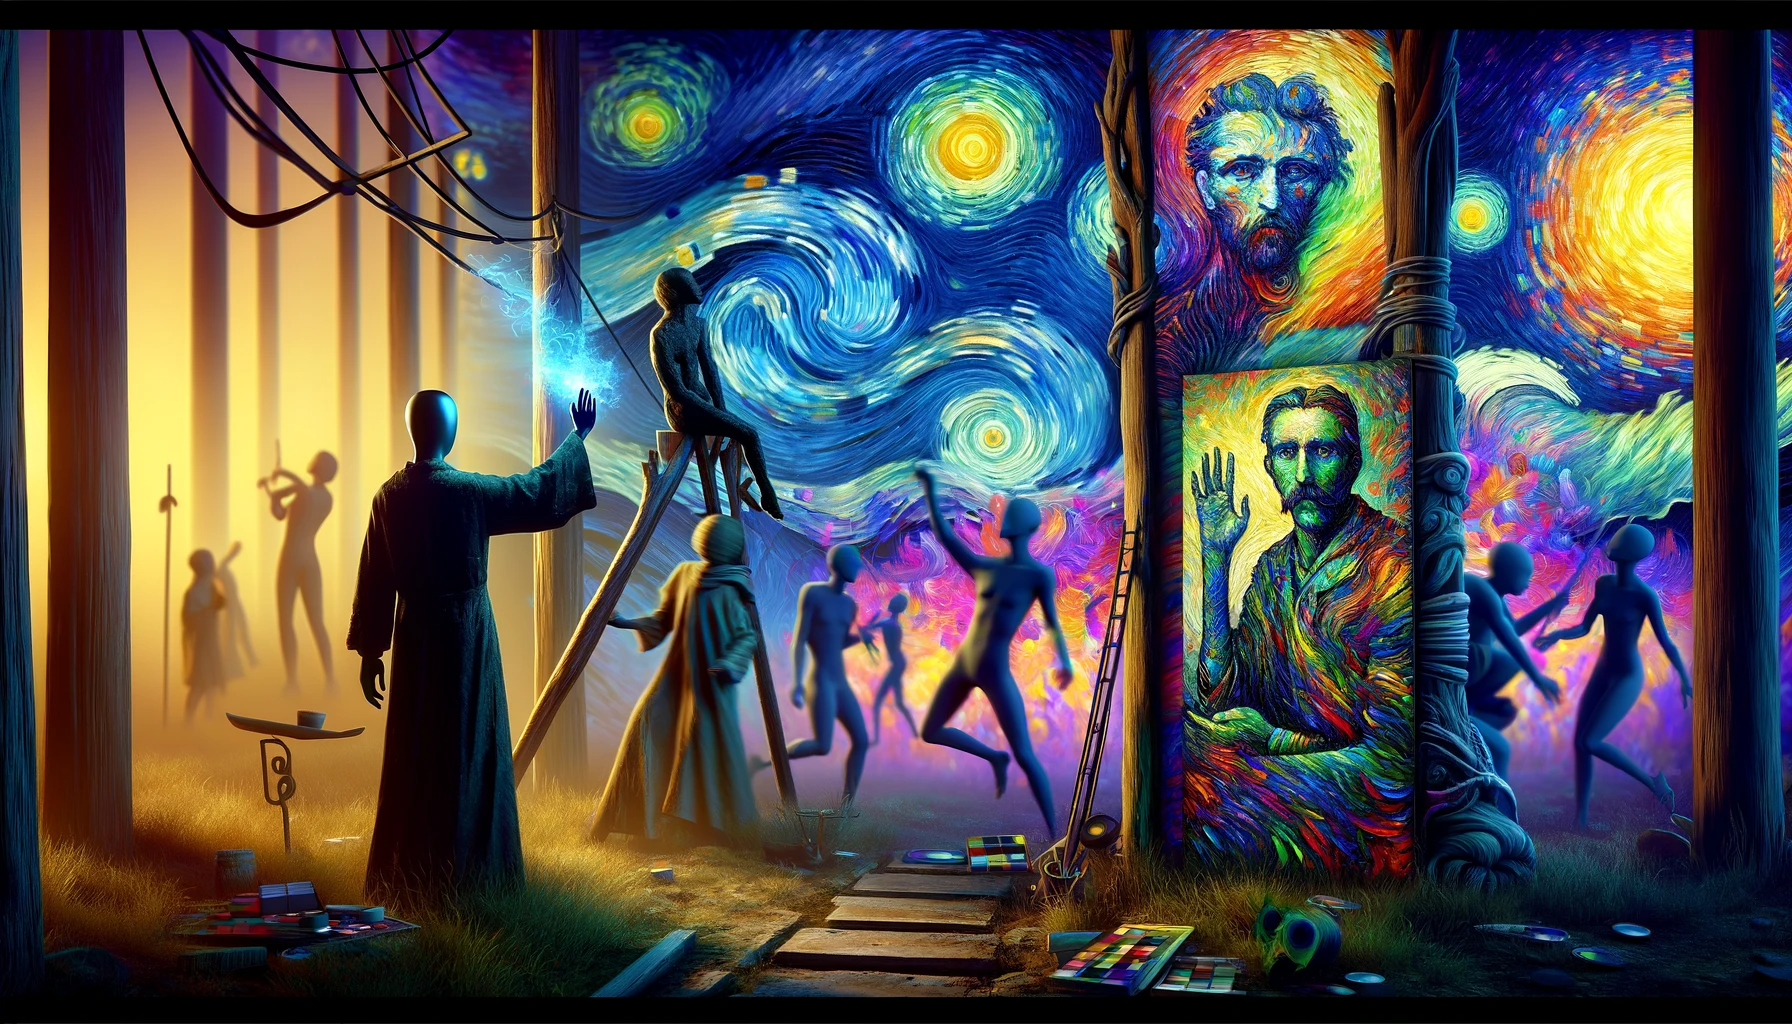
\includegraphics[width=\textwidth]{totemBanner.png}
    \caption{The spirit of the Totem platform.}
    \vspace{0.1cm}
    \label{fig:spiritofTotem}
\end{figure}

\subsection{ Introduction to the Totem Platform}

\subsubsection{Objective}

The Totem platform is designed to re-imagine digital art by integrating Artificial Intelligence and Augmented Reality into a single, interactive experience.
Positioned at the intersection of AI-driven creativity and immersive media, the Totem enables users to transform simple sketches into intricate, animated AR experiences.
% By combining generative and motion models, the Totem goes beyond static images, offering an intuitive and accessible way for creators to bring digital art to life.
The Totem goes beyond static images by combining generative and motion models, offering an intuitive and accessible way for creators to bring digital art to life.
This platform not only advances the possibilities for interactive storytelling but also supports the research objective of exploring low-signaling, high-possibility affordances, empowering users to create and engage with minimal input.

\begin{figure}[!h]
    \centering
    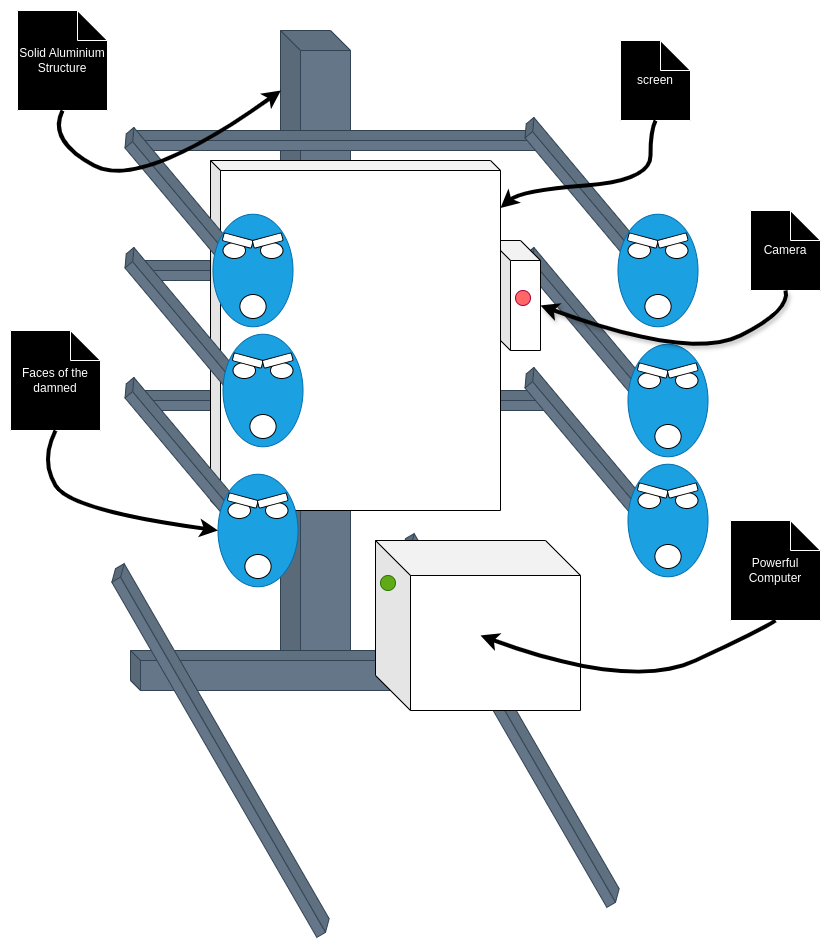
\includegraphics[width=\textwidth/2]{totem.drawio.png}
    \caption{Simplified representation of the Totem platform.}
    \vspace{0.1cm}
    \label{fig:totemImage}
\end{figure}

\subsubsection{Contextual Background}
Traditional digital art creation can be time-consuming and often requires substantial technical expertise, particularly for tasks like adding realistic motion or generating intricate visual details.
Animation, in particular, has remained a skill-intensive process, limiting accessibility for many potential creators.
The Totem addresses these limitations by simplifying the creative process through AI-enabled automation, transforming initial sketches into detailed art that responds to user movements.
This approach democratizes digital art, making advanced, interactive content creation accessible to a broader audience and reducing the need for specialized skills.

\subsubsection{Technologies Overview}
The core technologies behind Totem include SDXL Turbo\cite{sauer2023adversarial}, First Order Motion\cite{Siarohin_2019_NeurIPS}, and the General Operating System for Augmented Interfaces (GOSAI)\cite{gosai2022}.
SDXL Turbo, a state-of-the-art diffusion model by Stability AI, interprets users' sketches and enhances them with rich visual detail, transforming basic inputs into complex, artistically styled images.
The First Order Motion model animates these creations, adding realistic movements that elevate static images into dynamic, immersive characters.
Together, these AI models enable users to engage with their art in real-time.
At the foundation of Totem lies the GOSAI framework. The General Operating System for Augmented Interfaces, developed at \textbf{the DeVinci Innovation Center} streamlines the development of Augmented Interfaces, allowing developers to deploy and scale digital content as an extension of the physical world.
With these technologies, the Totem achieves a unique combination of AI and AR, exploring how digital art is created and experienced.

\subsection{ System Architecture and Workflow}

\subsubsection{Workflow Overview}
The Totem platform follows a structured workflow designed to transform user sketches into animated, immersive AR experiences.
The process flows through two primary apps—Generation and Animation—each responsible for distinct parts of the user interaction.
The Generation App enables users to create sketches in AR and stylize them in real time, while the Animation App brings these images to life with dynamic movement.
This sequential workflow begins with the \textbf{Sketch Input} \& AI Transformation stage, followed by Animation in AR.

\begin{itemize}
    \item \textbf{Generation App:} User sketches are processed by SDXL Turbo on a remote endpoint to create detailed portraits, which are updated in real time as the user draws.
    \item  \textbf{Animation App:} Generated portraits are animated with the First Order Motion model, enabling users to manipulate these images interactively in an AR environment.
\end{itemize}
This high-level division of tasks ensures Totem’s seamless performance by offloading resource-intensive tasks and optimizing real-time responsiveness.

\subsubsection{System Architecture}

The Totem platform's architecture leverages the General Operating System for Augmented Interfaces, to manage efficient data flow and resource allocation across its components.
At the heart of this architecture, the Redis\cite{carlson2013redis} database plays a crucial role, acting as a shared data cache to store and retrieve information across threads.
This enables GOSAI to separate the various system drivers, applications, and compute resources while maintaining fast, synchronized data access.
Redis allows drivers responsible for collecting and processing user inputs to interact seamlessly with the Totem’s generation and animation apps, ensuring that data is consistently available without duplication.
This architecture, shown in figure \ref{fig:diagtotem}, enhances the responsiveness of the platform by streamlining data sharing and distributing workloads, allowing the Totem to handle complex interactions smoothly across devices and contributing to the overall efficiency and scalability of Totem’s AR experience.

\begin{figure}[h!]
    \centering
    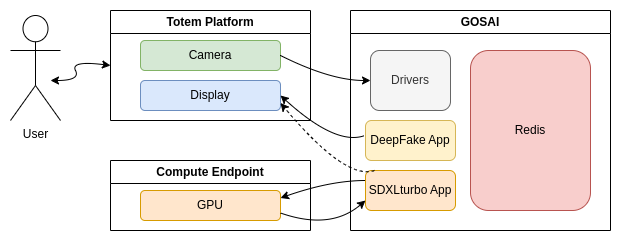
\includegraphics[width=\textwidth]{totemDiag.drawio.png}
    \caption{Architecture diagram of the AI Totem platform.}
    \vspace{0.1cm}
    \label{fig:diagtotem}
\end{figure}

\subsubsection{ Generation App}

This app allows users to create and stylize digital portraits in real time.
Users start by drawing a sketch, which, along with a style prompt, is sent to the SDXL Turbo model via a remote endpoint.
Since SDXL Turbo is a high-memory model, processing is offloaded to a remote server.
The resulting AI-generated images evolve as the user refines the sketch, enabling rapid iteration and exploration within a controlled, visually stable environment as shown in figure \ref{fig:imgenapp}.
To avoid flickering, the model uses a fixed seed for noise generation, ensuring consistency in the generated output.
This approach allows users to experiment freely with image creation, adjusting both content and style until satisfied.

\begin{figure}[!h]
    \centering
    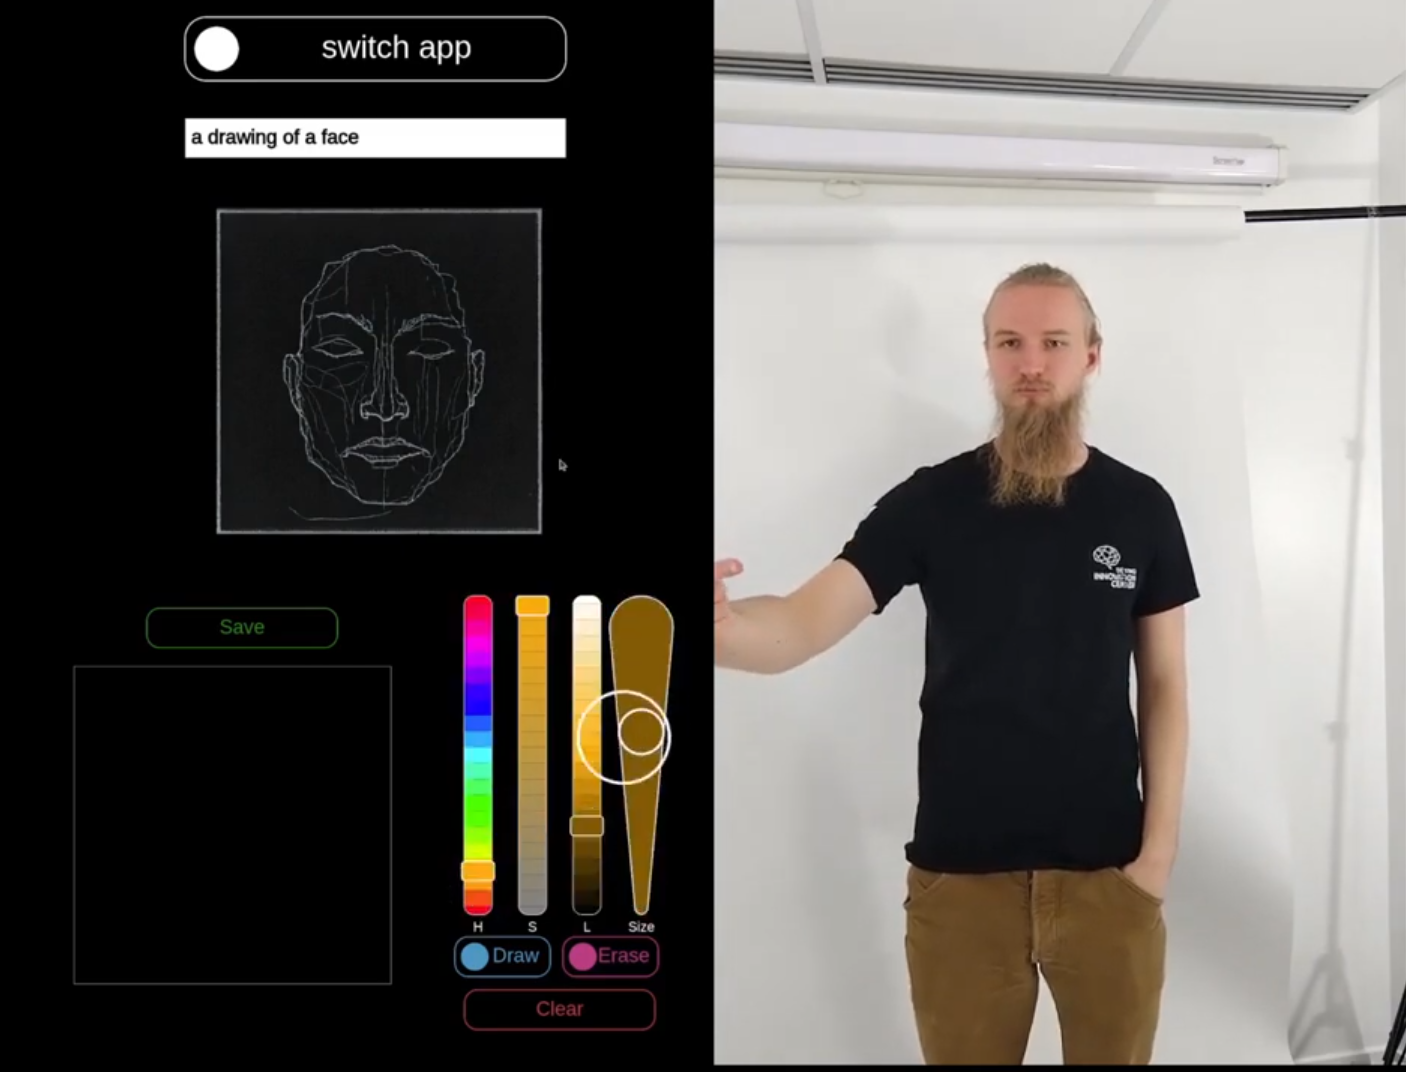
\includegraphics[width=\textwidth/2]{sdxl0.png}
    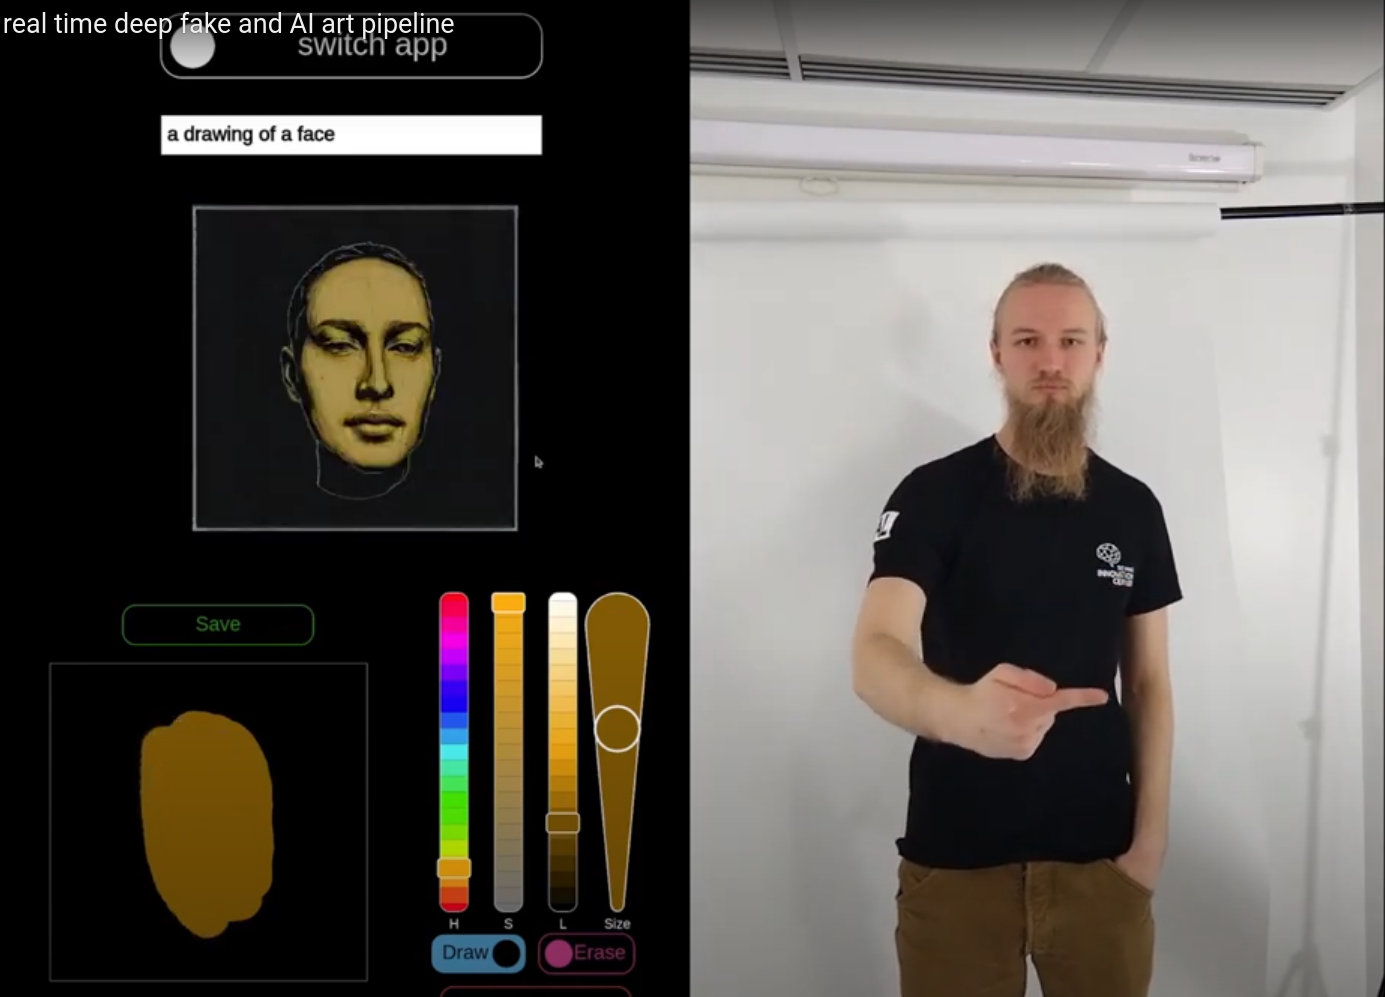
\includegraphics[width=\textwidth/2]{sdxlapp.png}
    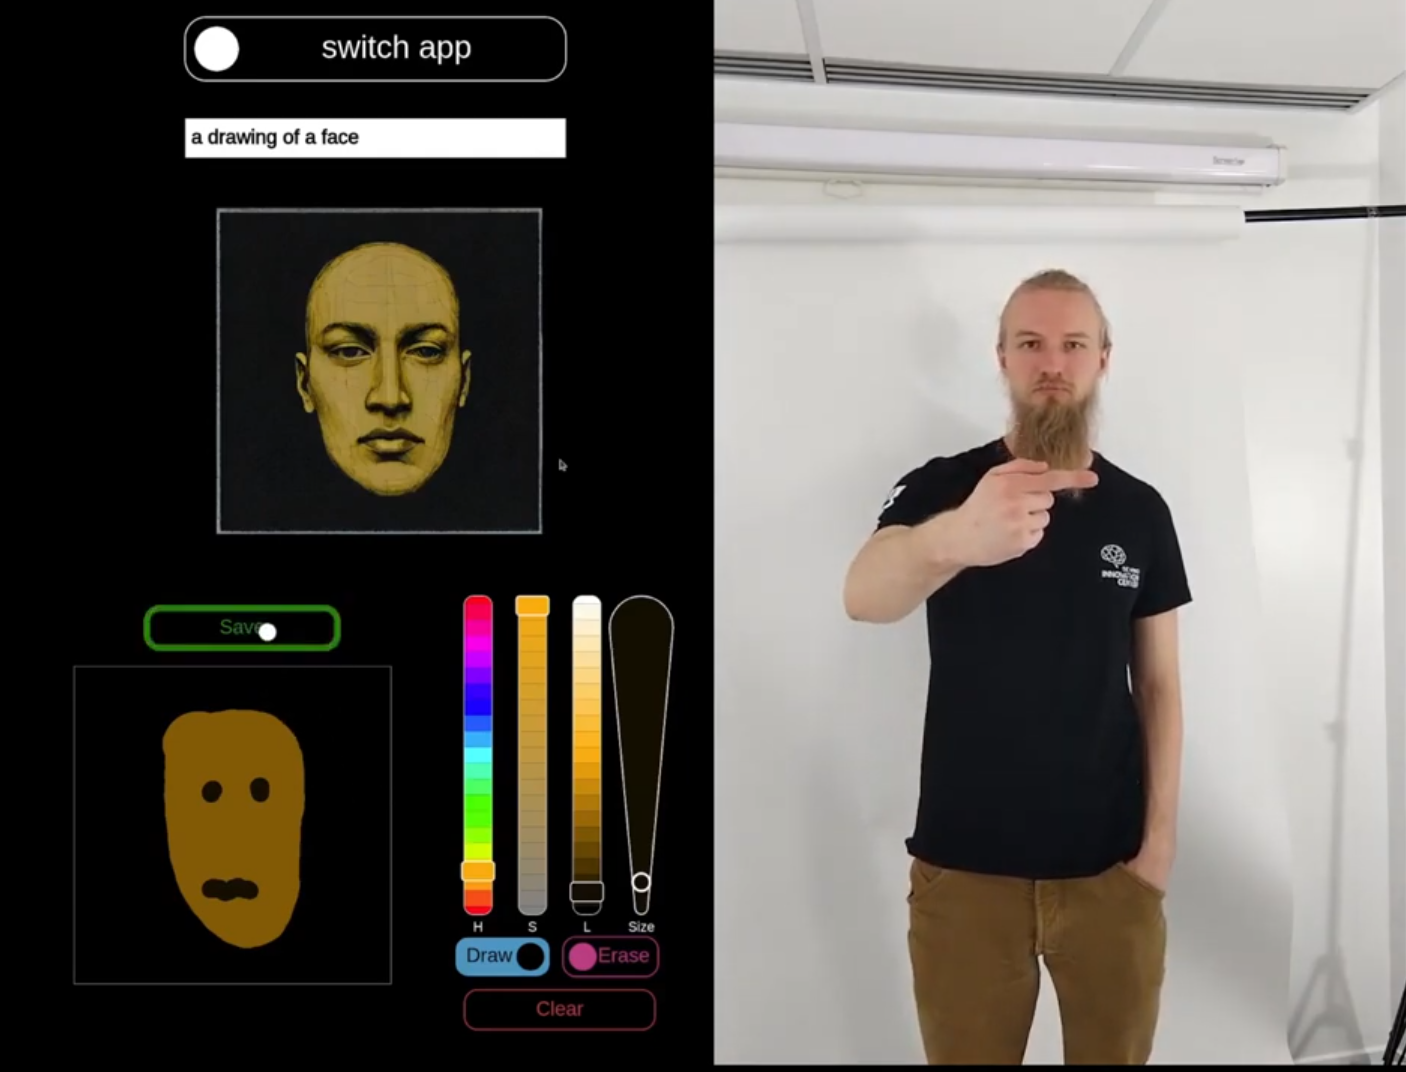
\includegraphics[width=\textwidth/2]{sdxl2.png}
    \caption{Overview of the image generation app.}
    \vspace{0.1cm}
    \label{fig:imgenapp}
\end{figure}

\subsubsection{Animation App}

Once an image is generated, users can animate it using the Animation App.
This app loads the created or pre-existing portraits and animates them with the First Order Motion model, which has low computational requirements, making real-time processing feasible directly on the device.
Powered by the GOSAI framework, the Animation App interprets user gestures or head movements, linking them to character animations within the AR environment, as shown in figure \ref{fig:deepfakeapp}.
This component enables fluid interaction, allowing users to manipulate and engage with their digital characters dynamically, bringing a layer of immersion and expressiveness to the experience.

\begin{figure}[!h]
    \centering
    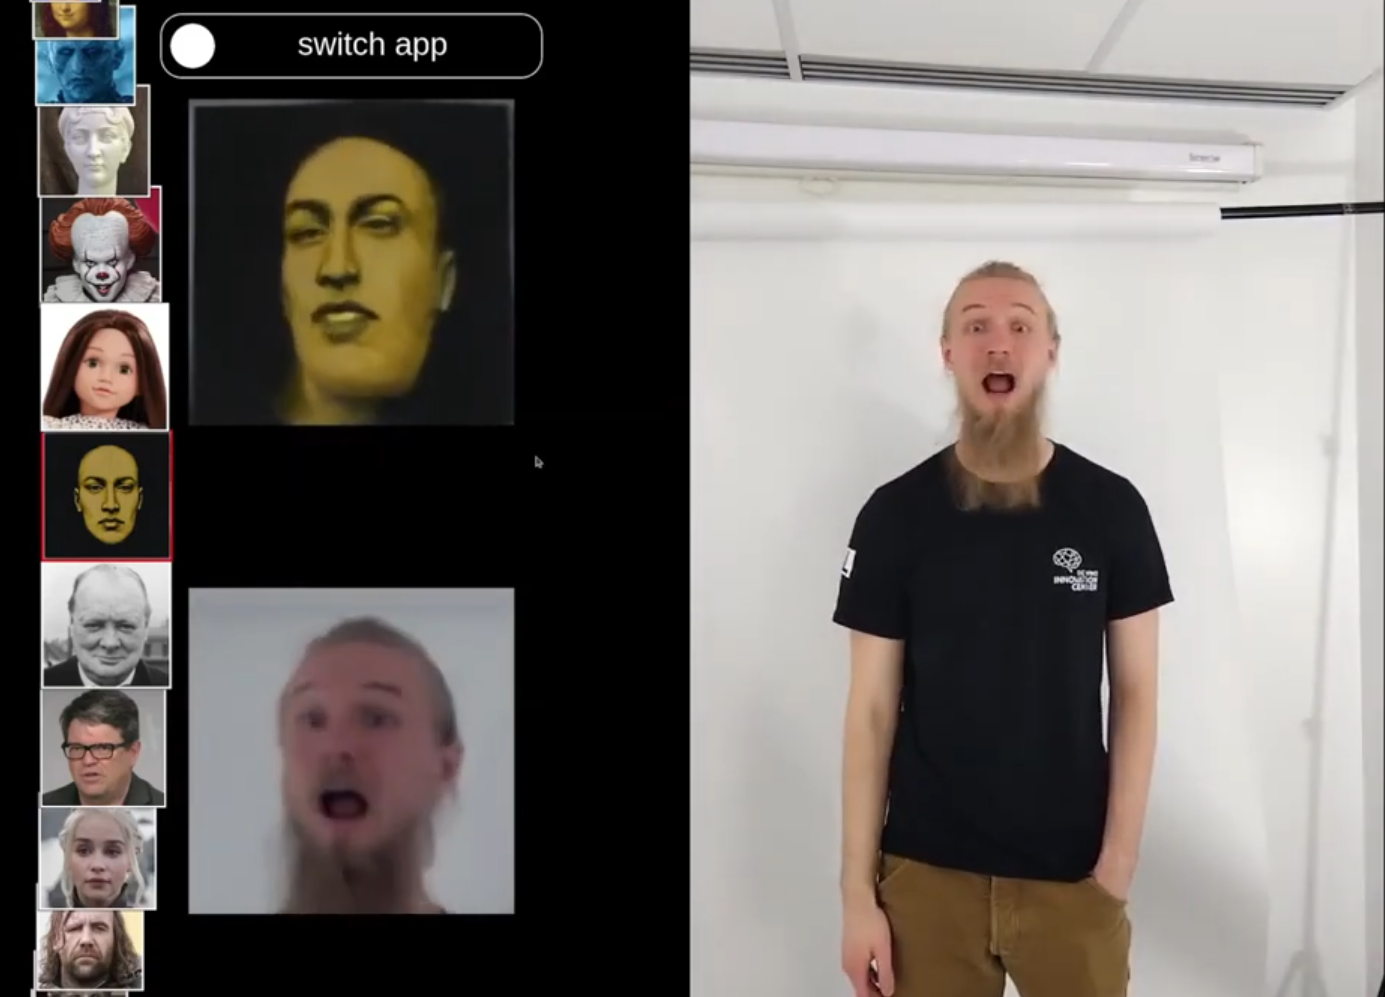
\includegraphics[width=\textwidth/2]{deepfakeapp.png}
    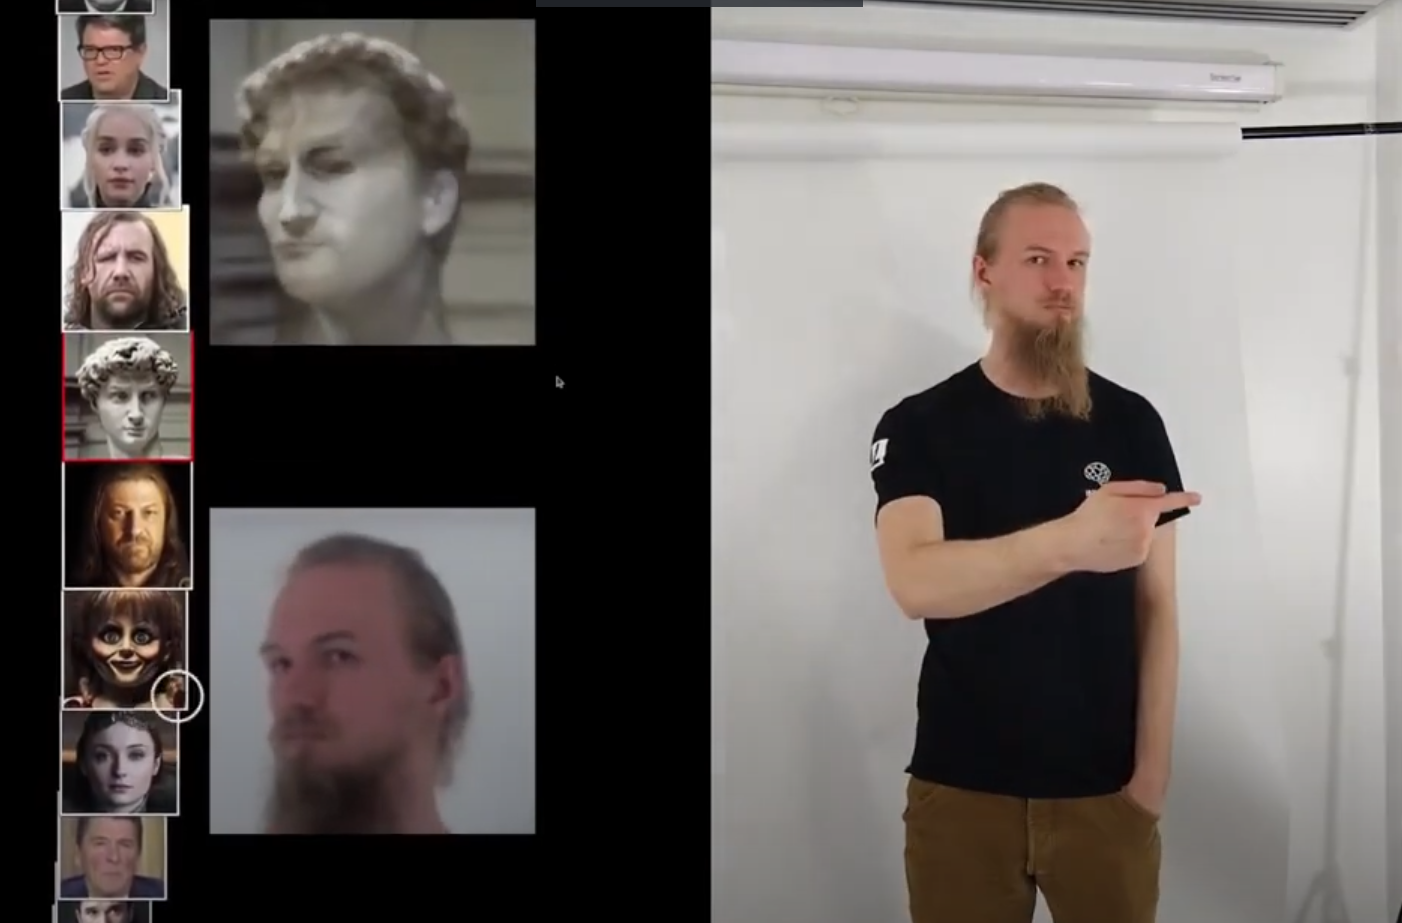
\includegraphics[width=\textwidth/2]{anim0.png}
    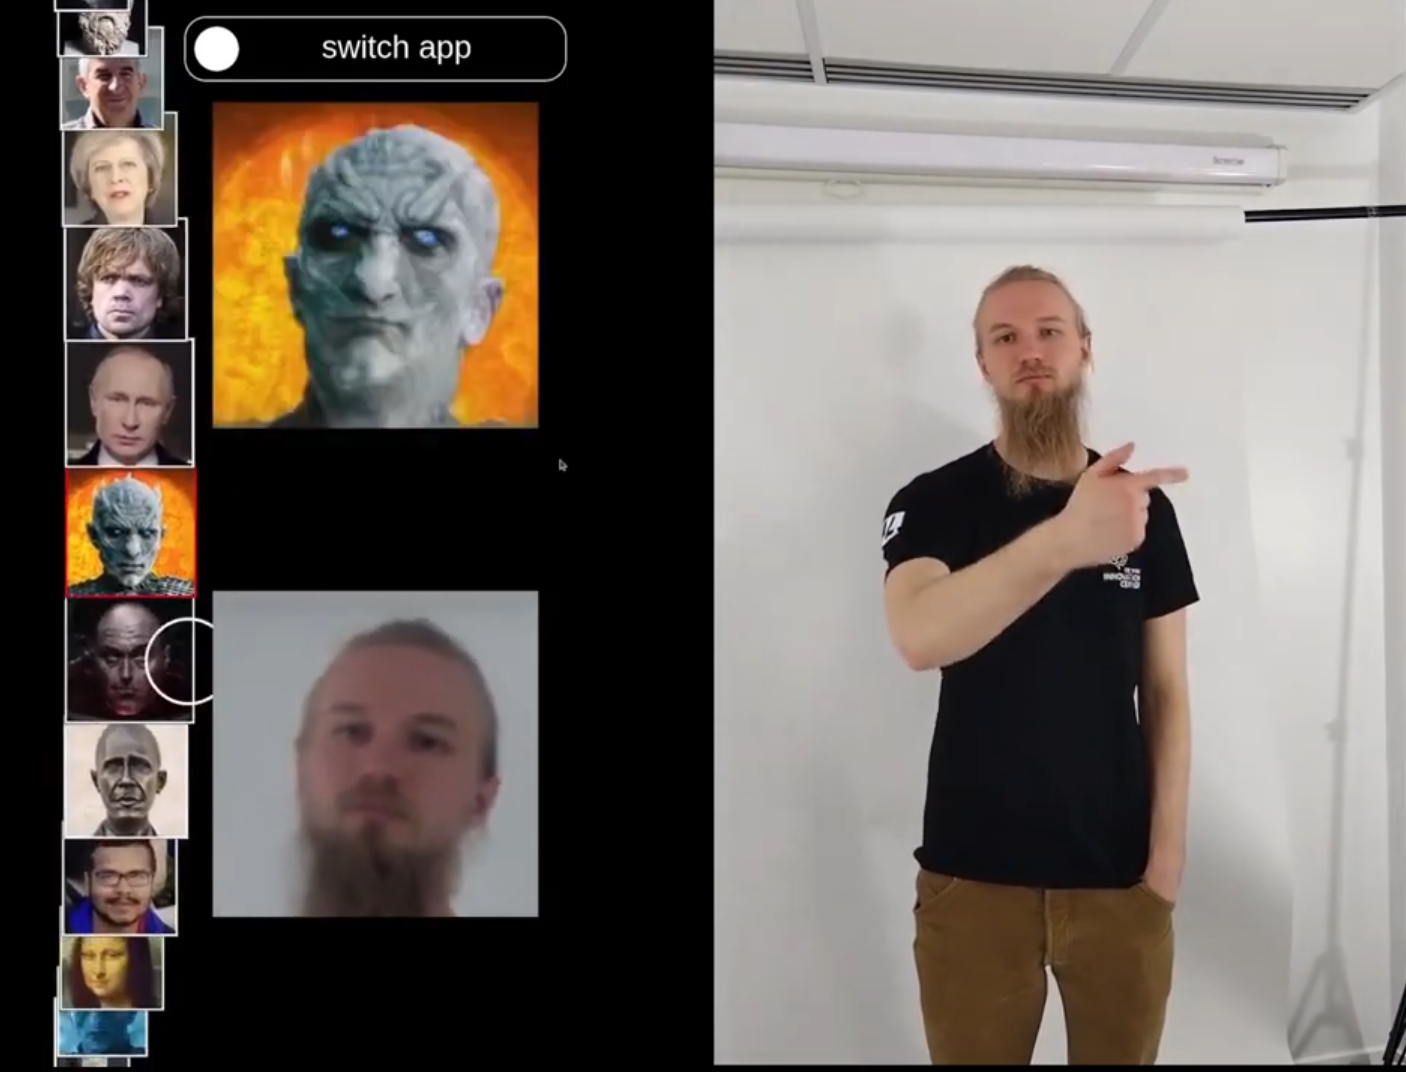
\includegraphics[width=\textwidth/2]{anim1.png}
    \caption{Overview of the animation app.}
    \vspace{0.1cm}
    \label{fig:deepfakeapp}
\end{figure}

By separating the tasks between the Generation and Animation apps, the Totem achieves a balanced system architecture that maintains both high-quality image generation and real-time interactivity.
The GOSAI framework integrates these components into a unified AR platform, providing users with a seamless experience.
This division of compute allows the Totem to handle both remote processing for high-quality imagery and on-device animation, optimizing for performance and interactivity within a resource-efficient design.

\subsection{Transforming Sketches into Detailed Images with SDXL Turbo}

The transformation of a user’s sketch in AR, into a photorealistic, AI-generated image within the Totem platform is achieved through SDXL Turbo\cite{sauer2023adversarial}, an advanced diffusion model optimized for speed and detail.
Building on the original SDXL 1.0 architecture, SDXL Turbo enhances input sketches with intricate textures and refined visual elements, turning rough concepts into highly detailed digital art.
This model uses Adversarial Diffusion Distillation (ADD), a technique that enables high-quality image generation with minimal computational steps, allowing the Totem to deliver fast, visually rich results.

\subsubsection{Efficiency Considerations}
SDXL Turbo’s efficiency stems from the Image-to-Image Diffusion technique, which progressively refines the sketch with each diffusion step to add depth and realism.
Diffusion techniques iteratively refine noised inputs to finished outputs. This can create flickering in the output even though the input image is stable if the noising is too random.
A critical feature of our process is the use of a constant seed during image noising, ensuring that the resulting images remain stable and consistent as the user draws, avoiding unwanted flickering between samples.
The ADD technique enables the model to produce high-fidelity images in one or two sampling steps, significantly reducing the typical processing time associated with diffusion models.
ADD leverages a combination of distillation and adverserial loss that enables a smaller student model to perform as well as a bigger teacher model, as shown in figure \ref{fig:sdxlarchitecture}.
This enables the Totem to generate images in real time, ensuring a seamless creative flow even for complex, photorealistic details.

\begin{figure}[!h]
    \centering
    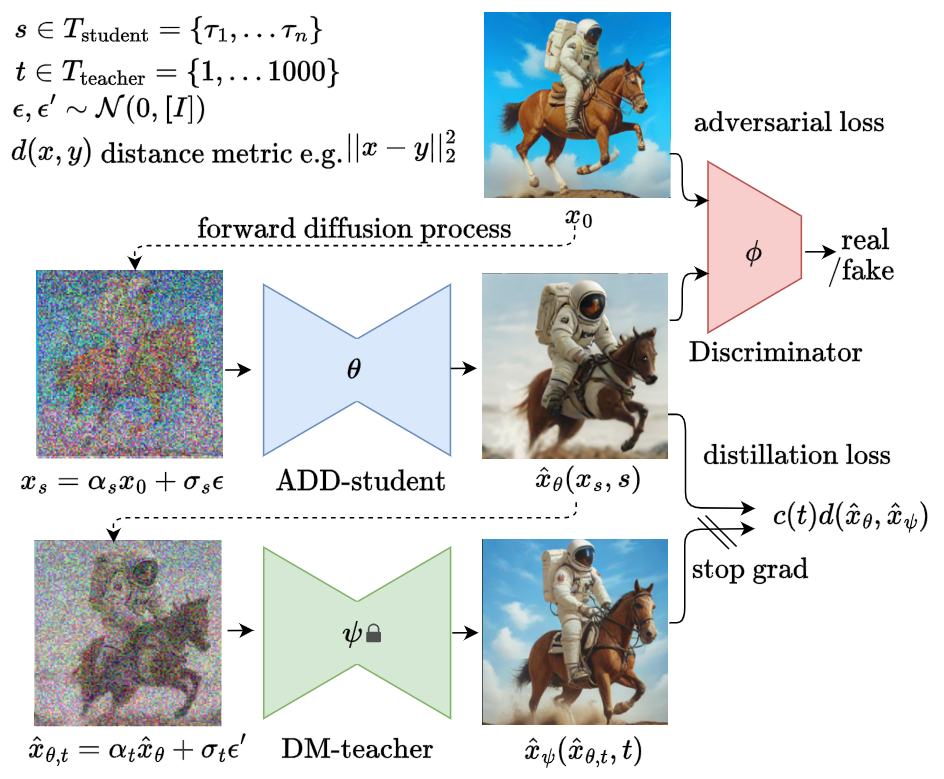
\includegraphics[width=\textwidth/2]{sdxlarchitecture.png}
    \caption{Architecture of the SDXL Turbo model.}
    \vspace{0.1cm}
    \label{fig:sdxlarchitecture}
\end{figure}

\subsubsection{User Perspective}
For creators, SDXL Turbo transforms the Totem into a dynamic tool for rapid experimentation and engagement.
The near-instantaneous feedback allows users to see their ideas rendered in detail as they sketch, encouraging iterative design and exploration.
With the ability to modify style and content on the fly, users can experiment by turning a simple sketch into various artistic interpretations—such as changing the character from a man in a hat to a dog or a cat in a hat.
The possibilities offered by prompt conditioning are shown in figure \ref{fig:sdxlpainting}.
This adaptability not only enhances the user experience but also promotes creative freedom, making digital art creation accessible and highly interactive.

\begin{figure}[h!]
    \centering
    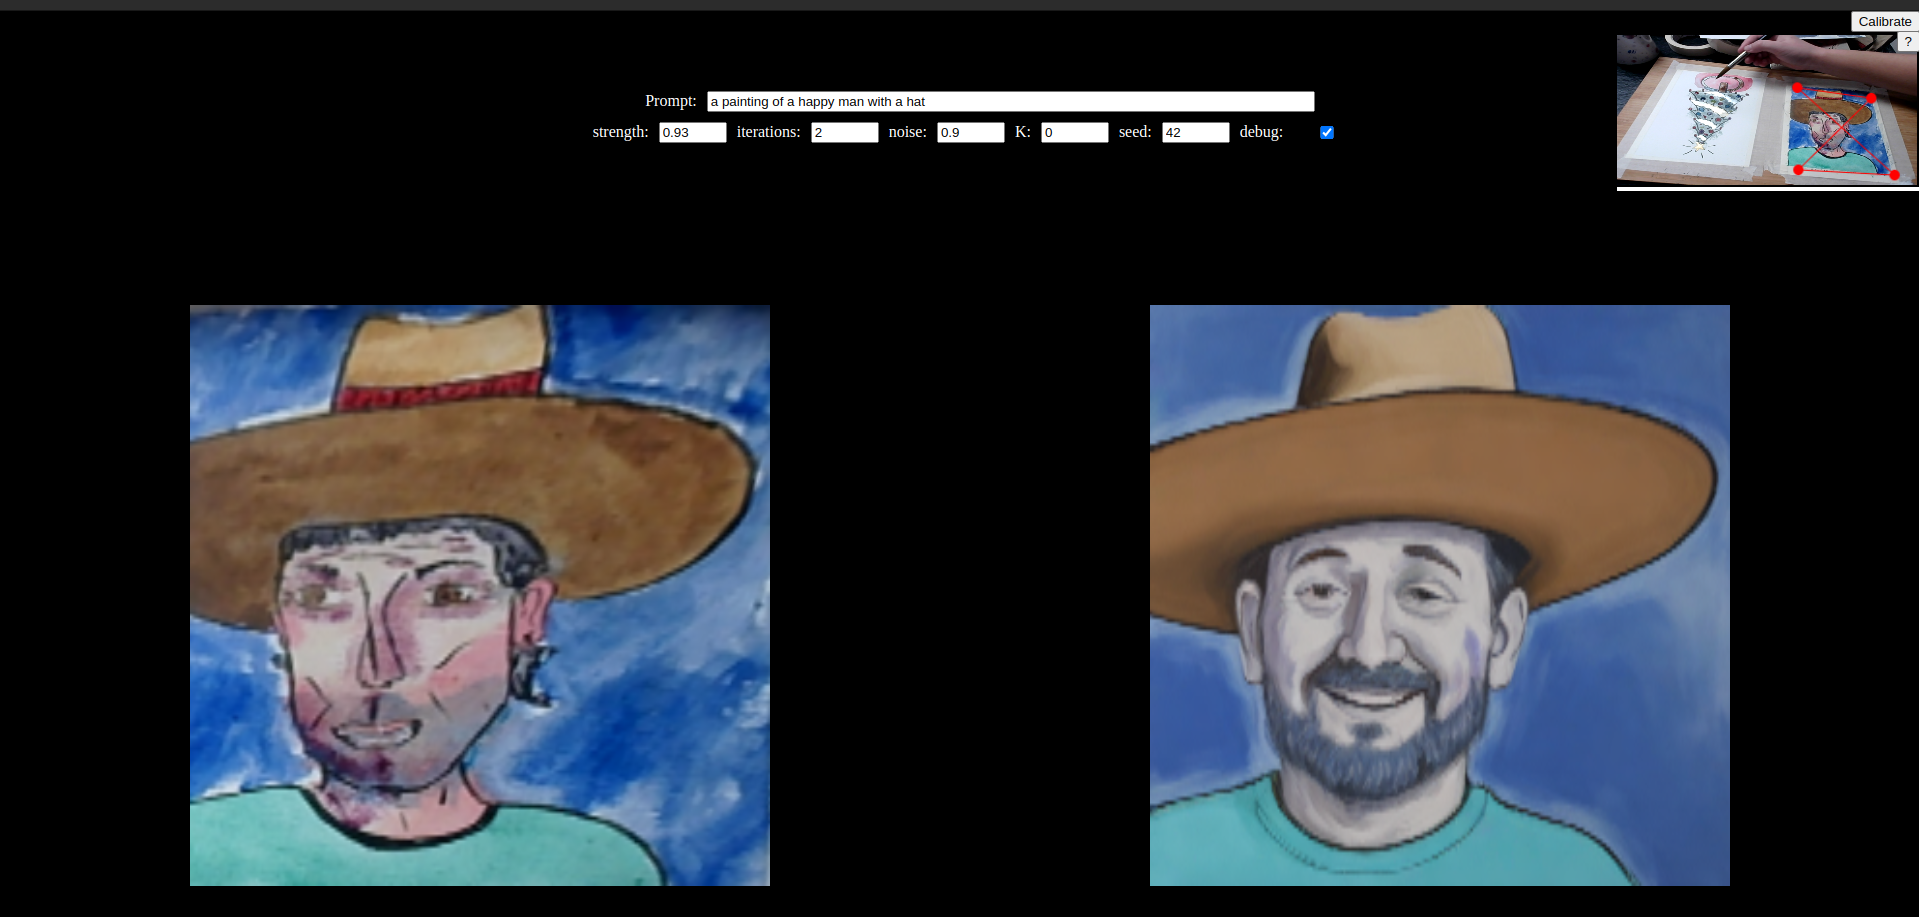
\includegraphics[width=\textwidth/3]{HatManhappy.png}
    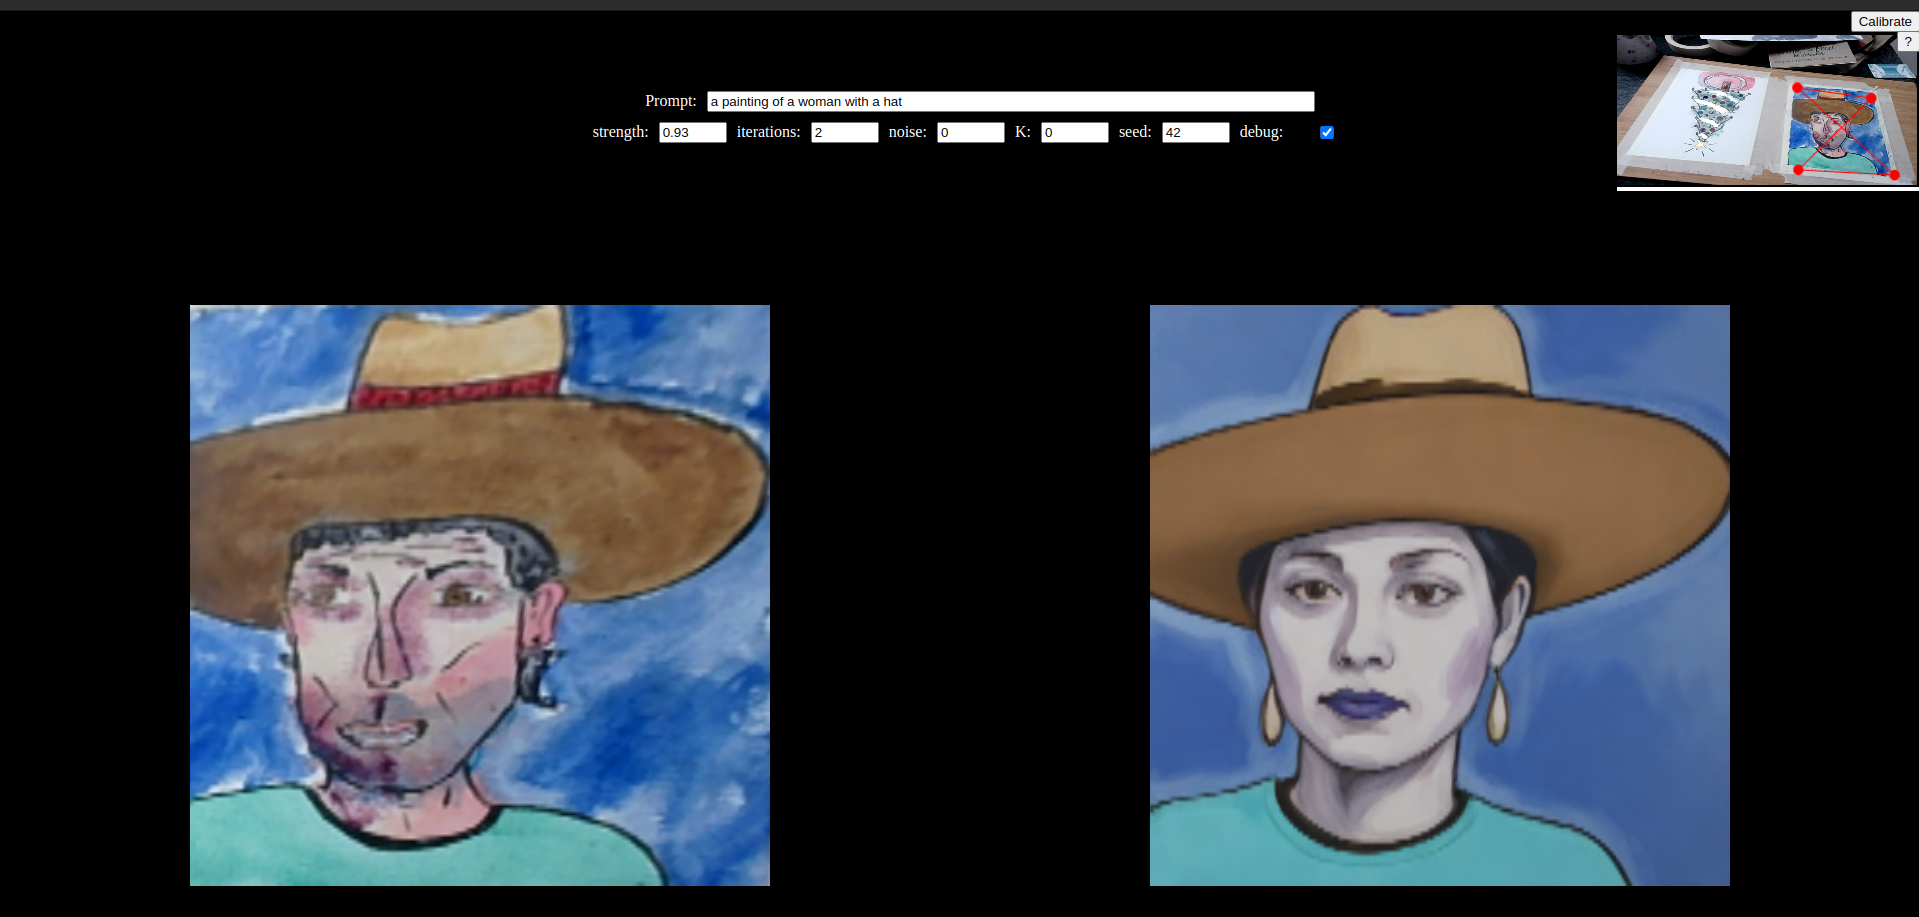
\includegraphics[width=\textwidth/3]{HatManwoman.png}
    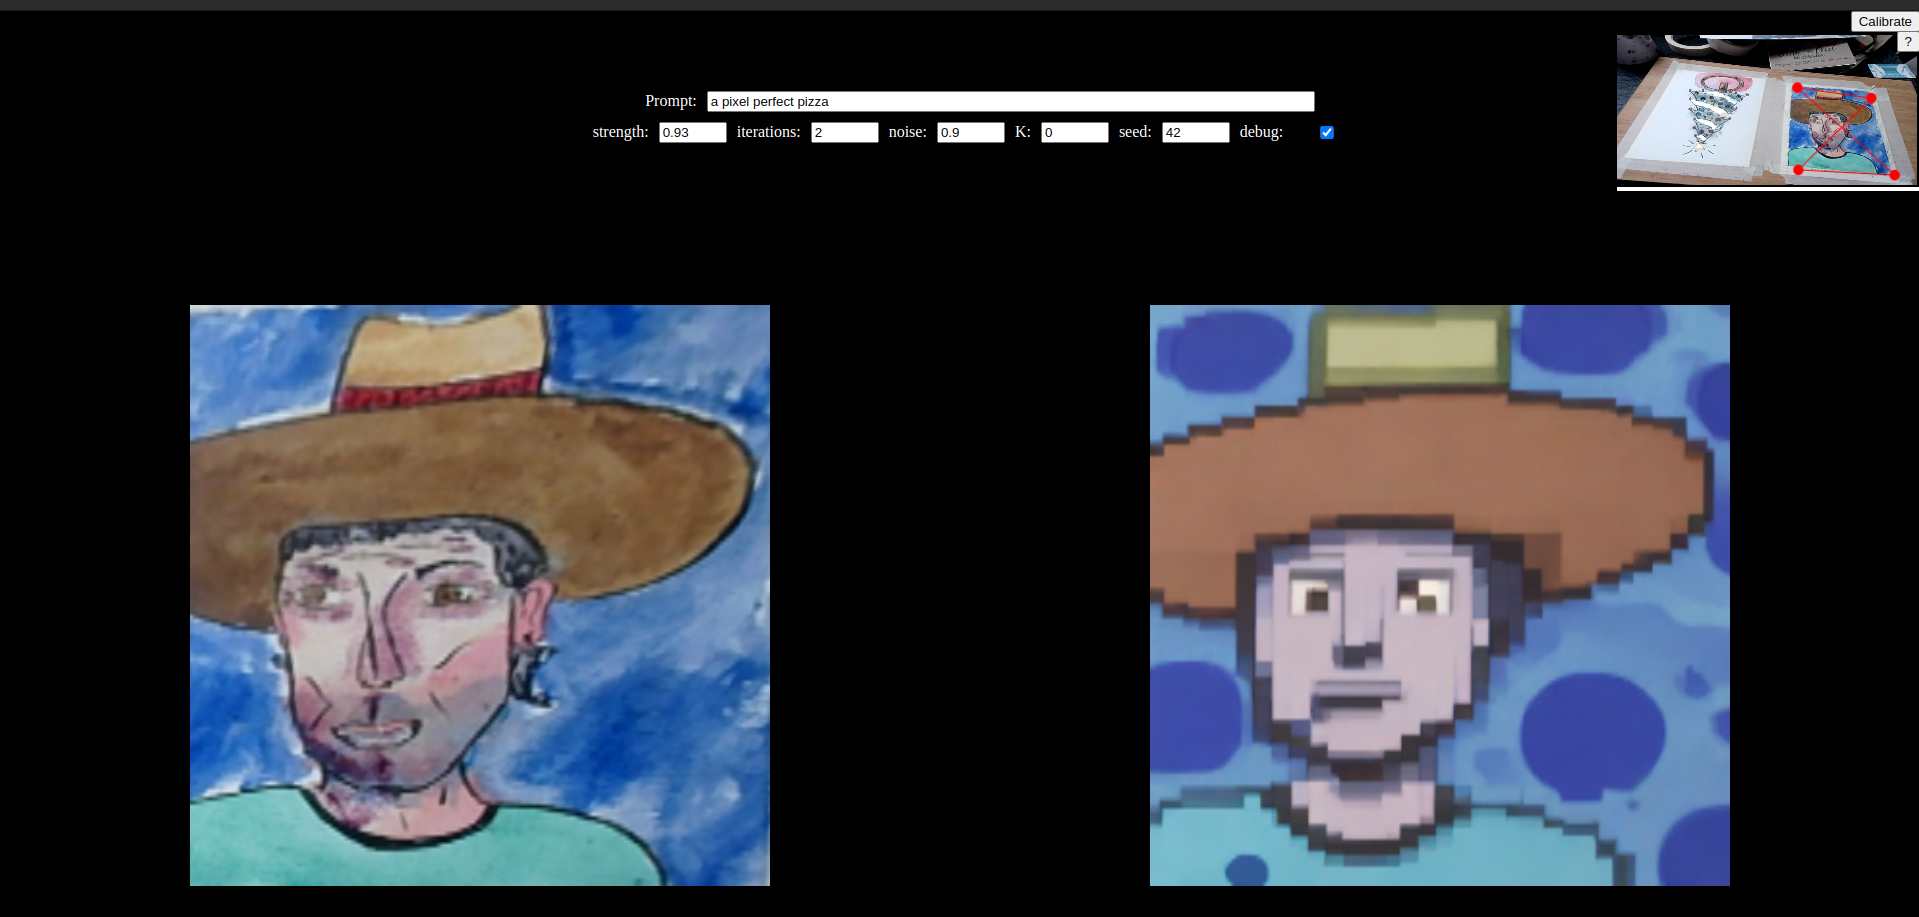
\includegraphics[width=\textwidth/3]{HatMancubes.png}
    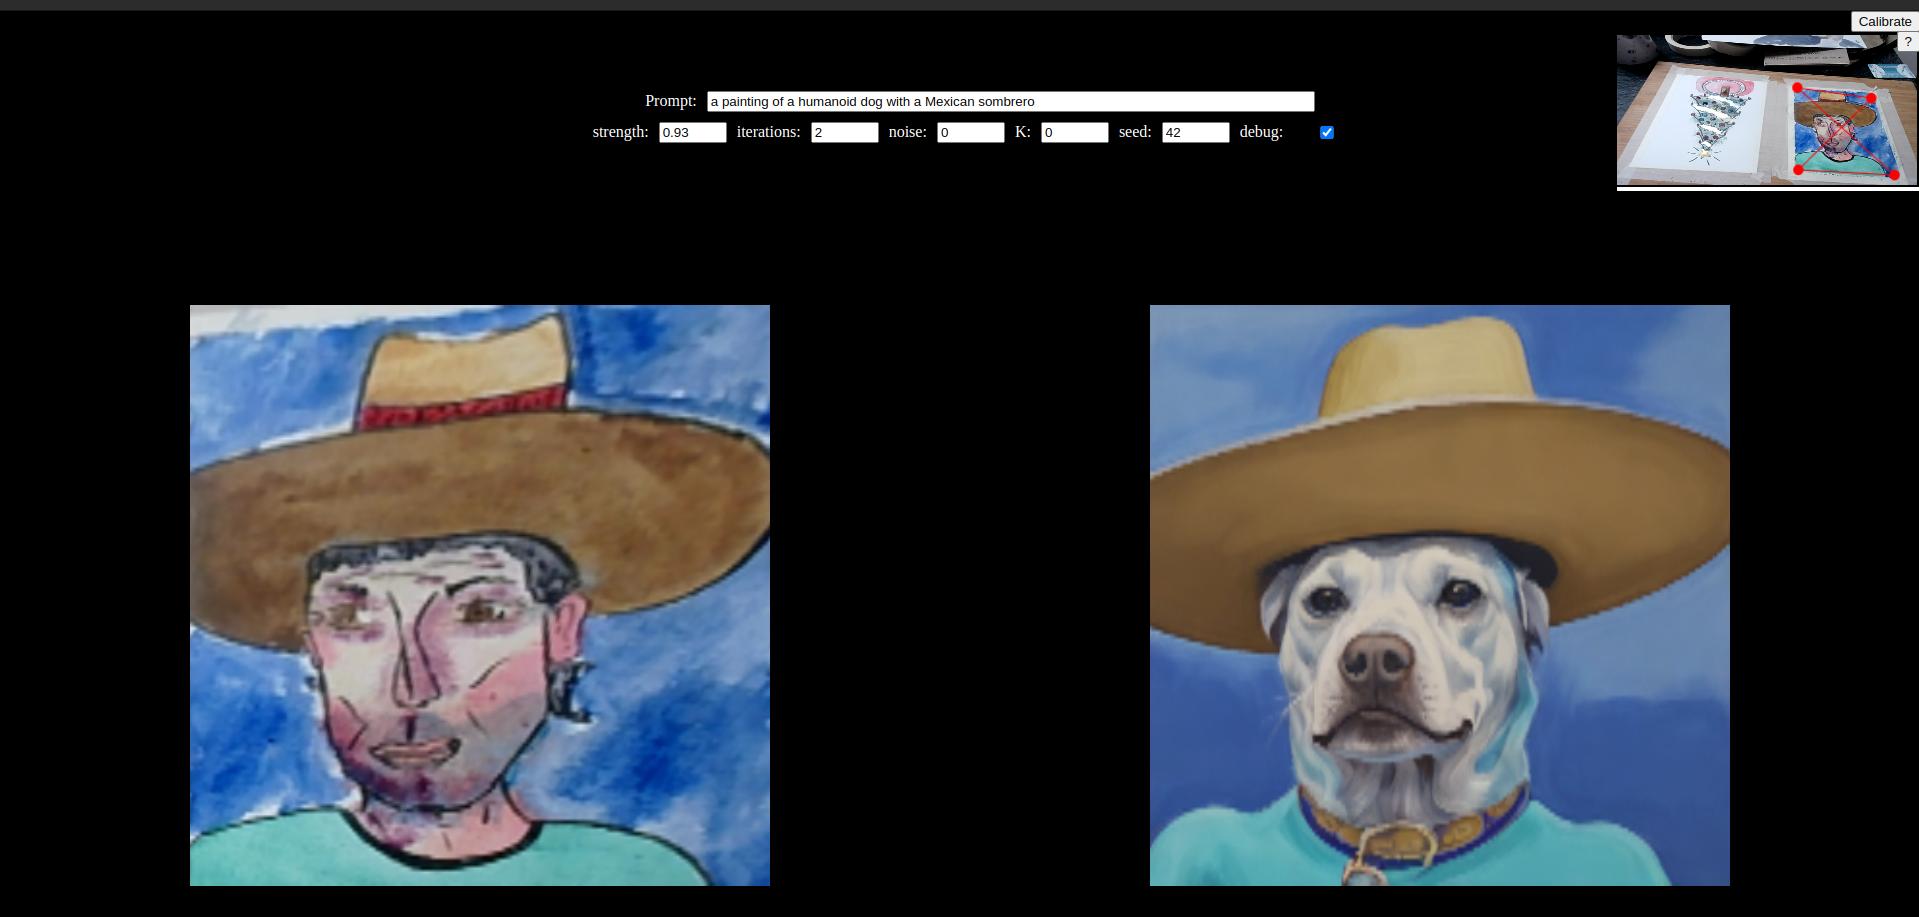
\includegraphics[width=\textwidth/3]{HatManDog.png}
    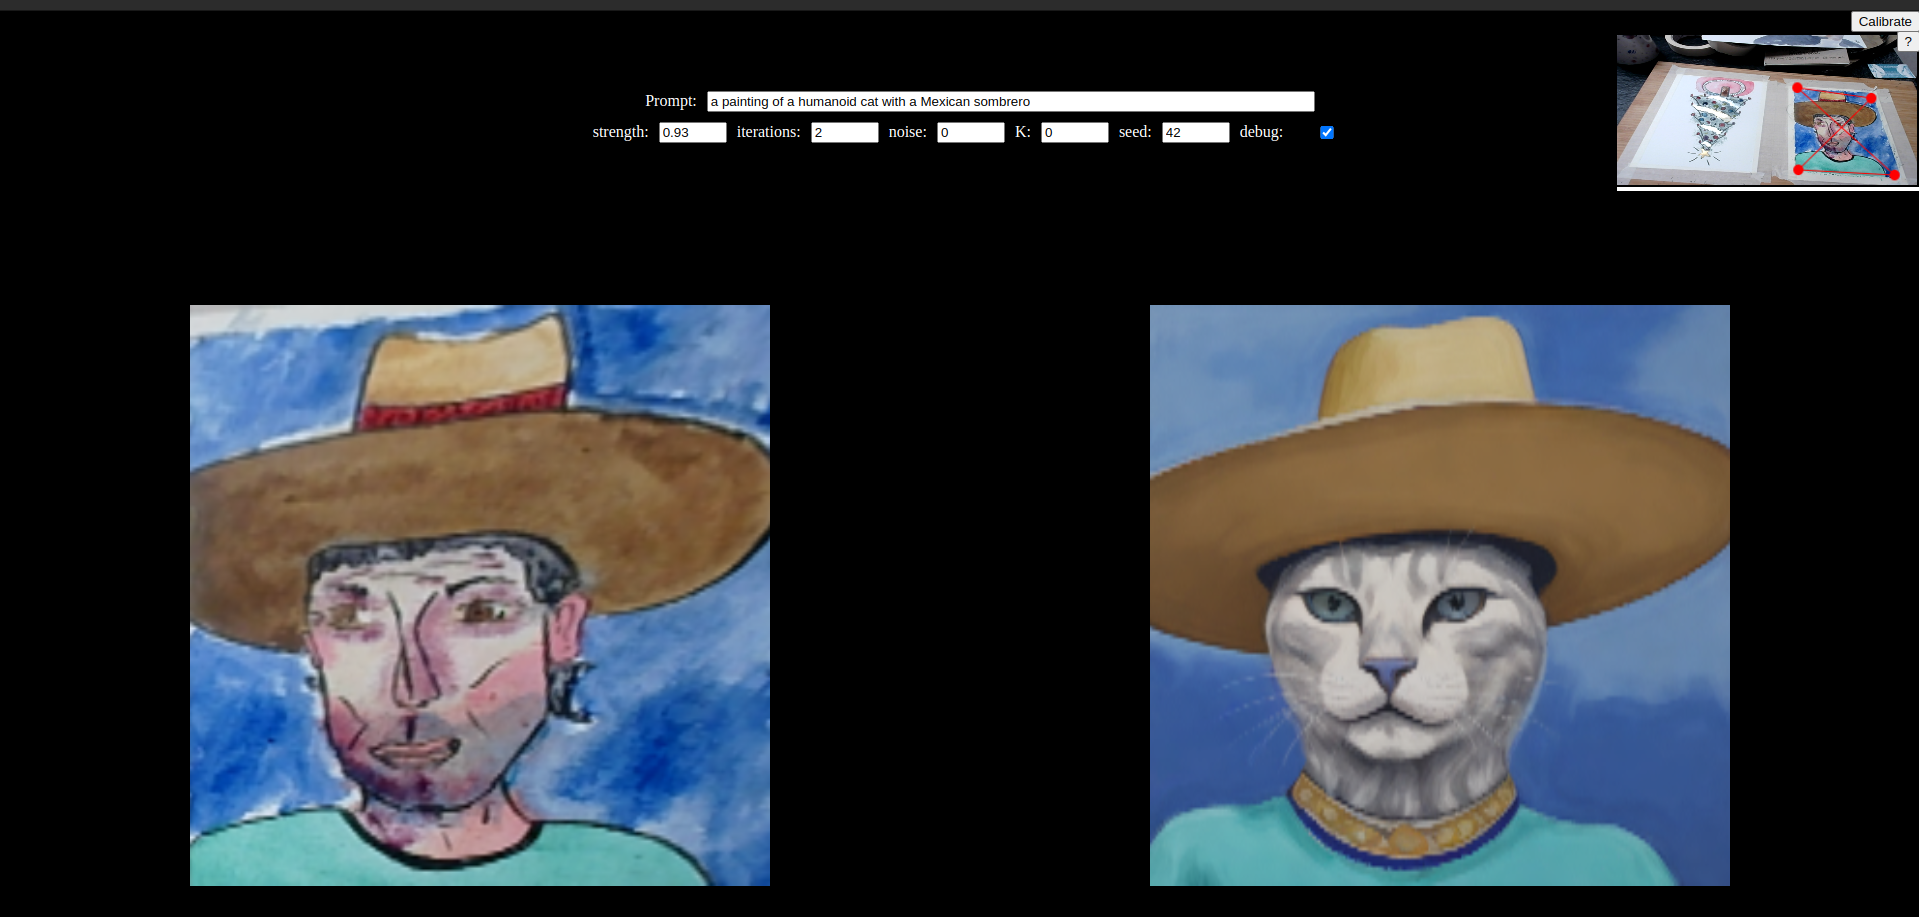
\includegraphics[width=\textwidth/3]{HatManCAT3.png}
    \caption{SDXL Turbo-generated images based on simple painting.}
    \vspace{0.1cm}
    \label{fig:sdxlpainting}
\end{figure}

\subsection{Animating Creations with First Order Motion}

\subsubsection{First Order Motion in the Totem}
The First Order Motion model\cite{Siarohin_2019_NeurIPS} brings AI-generated characters to life within the Totem platform by animating images with minimal computational overhead. 
Some animation methods such as deepfake techniques\cite{perov2020deepfacelab} rely on Generative Adversarial Networks (GANs)\cite{goodfellow2014generative}, which typically require training on specific source and target faces.
In contrast, the First Order Motion model uses a zero-shot approach to create animations from any input without prior exposure to the source material.
The model works by applying motion to keypoints in the image, generating realistic, dynamic expressions and movements that make the characters appear lively and responsive.
This efficient method is ideal for the Totem’s AR setting, as it enables interactive animations that naturally mimic the user.

\subsubsection{Performance Considerations}
First Order Motion offers significant performance advantages over GAN-based animation techniques.
While GANs are resource-intensive, hard to train and often need to be fine-tuned for specific images, the First Order Motion model operates by deforming keypoints and applying motion fields directly to existing images.
It extracts sparse motion trajectories from keypoints, transforming these into dense motion fields that animate the image.
This approach separates most of the complexity related to tracking the transformation of keypoints from the part of the model in charge of generating clean pictures (figure \ref{fig:firstorderarchitecture}).
The resulting lightweight design allows the Totem to animate characters in a resource-constrained environment, ensuring smooth performance in real-time without requiring a high-end GPU.

\begin{figure}[!h]
    \centering
    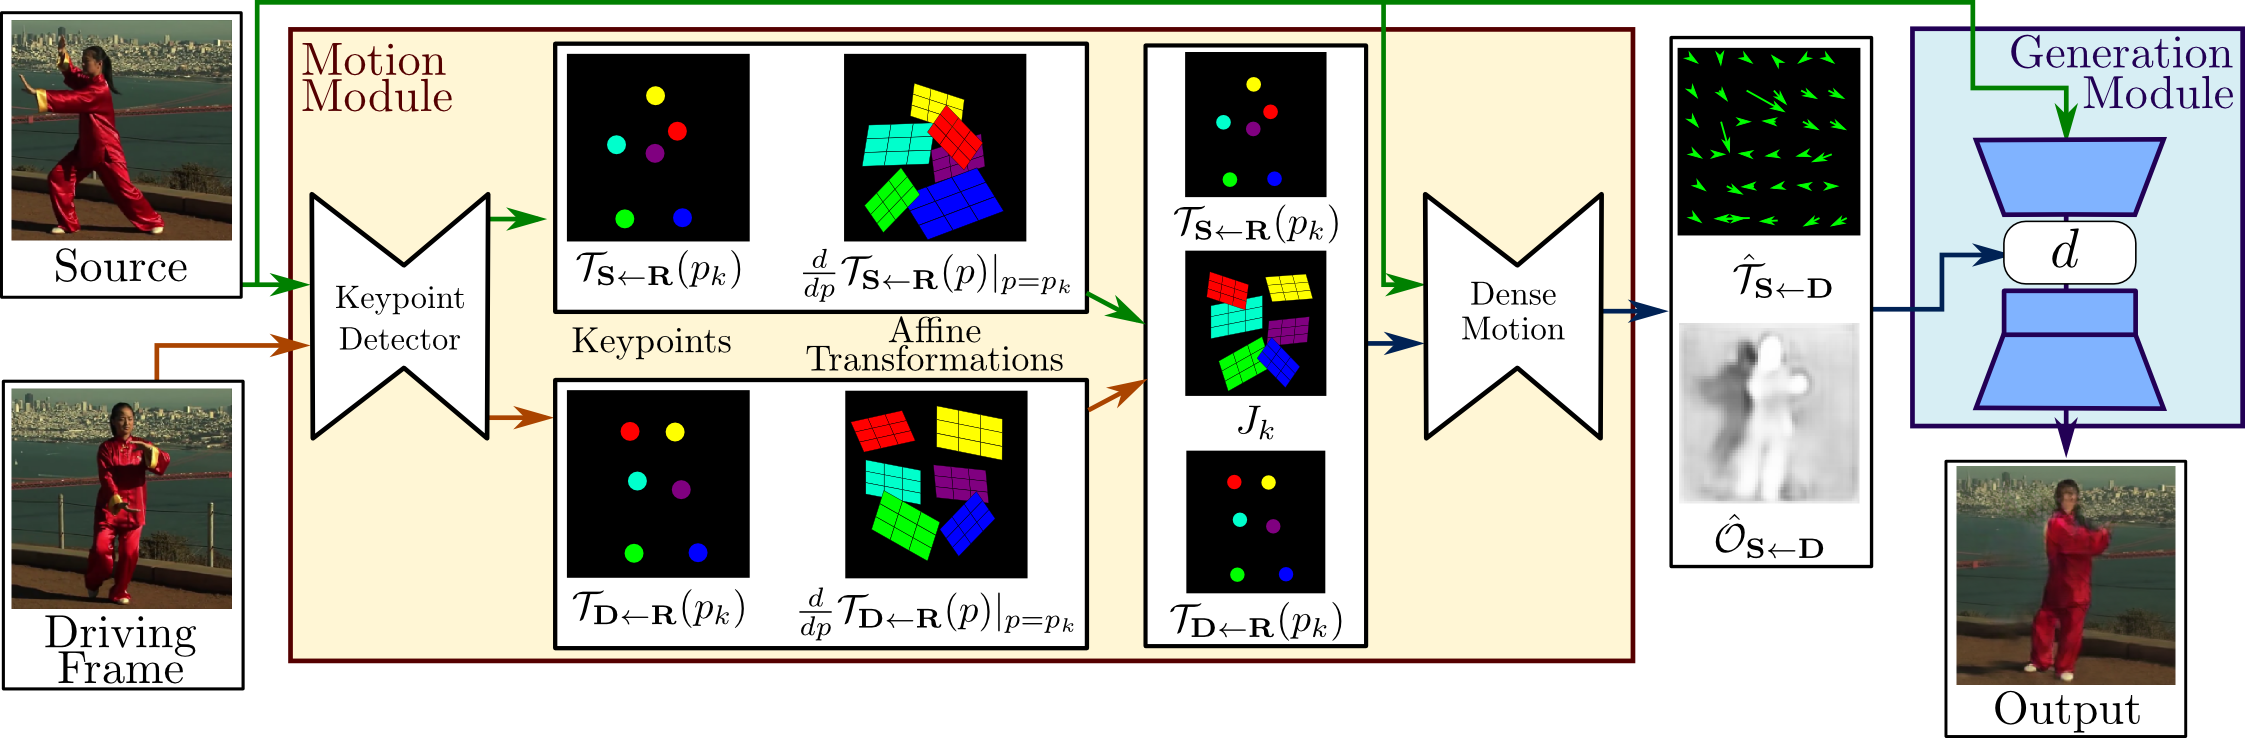
\includegraphics[width=\textwidth]{firstordermotion.png}
    \caption{Architecture of the First Order Motion Model.}
    \vspace{0.1cm}
    \label{fig:firstorderarchitecture}
\end{figure}

\subsubsection{User Interaction}
The inclusion of animation transforms the Totem experience from static viewing to immersive, interactive creation.
By animating AI-generated portraits, users can see their characters express emotions and respond to their movements.
This dynamic interaction makes the characters feel like a disguise for the user, enhancing user engagement.
The Totem’s approach empowers creators to bring their art to life, enriching storytelling and providing a uniquely immersive experience that adapts to real-world contexts.

\subsection{Implementation and Optimization Considerations}

\subsubsection{Framework Comparison}
To achieve efficient model inference within the Totem platform, various deep learning frameworks were evaluated, including PyTorch, TorchScript, and ONNX.
While PyTorch provides flexibility and ease of use during model development, it introduces computational overhead during inference.
TorchScript, an extension of PyTorch, offers incremental improvements by converting models into a more static form, but still lacks the aggressive optimizations needed for real-time applications.
ONNX (Open Neural Network Exchange) emerged as the optimal choice, allowing models to run with significantly lower latency and memory usage through optimizations like operator fusion and quantization.
ONNX’s static graph structure and cross-platform compatibility make it well-suited for performance-critical, resource-constrained applications, leading to a substantial increase in frames per second (FPS) and reduction in model size, as evidenced by benchmark results in table \ref{tab:frameworks}.

\begin{table}[!h]
\footnotesize%
\begin{center}
    \begin{tabular}{lccc}
    \toprule
    framework    & latency (ms)↓ & fps ↑  & model size (Mo)↓ \\
    PyTorch      & 0.069        & 14.3  & 716.4           \\
    Torch Script & 0.057        & 17.5  & 716.4           \\
    ONNX         & \textbf{0.026}& \textbf{38.46} & \textbf{279.1}           \\
    \bottomrule
    \end{tabular}
\end{center}
\caption{Comparison of different frameworks for the First Order Motion model inference.}
\label{tab:frameworks}
\end{table}

\subsubsection{Resource Allocation}
The Totem platform balances computational workload between remote endpoints and local processing to deliver high-quality, real-time AR interactions.
The SDXL Turbo model, which requires substantial memory and computational power, is hosted on a remote endpoint equipped with a Tesla V100 GPU.
This setup allows the model to operate with low latency, connecting over WebRTC to ensure seamless communication.
The First Order Motion model, by contrast, is lightweight enough to run directly on the device, operating within a dedicated GOSAI thread.
This distributed architecture allows the First Order Motion model to animate characters in real time, leveraging MediaPipe drivers to capture and process user movements, which are shared across Totem applications.

\subsubsection{GOSAI: The Backbone of AR Performance}
The General Operating System for Augmented Interfaces (GOSAI), is central to the Totem’s AR experience, providing a robust infrastructure that supports efficient data handling.% and processing across devices.
% Utilizing Redis for caching and data sharing, GOSAI separates tasks between drivers, applications, and compute resources, allowing the system to allocate resources dynamically.
The system allocates resources dynamically by utilizing Redis for caching and data sharing while GOSAI separates tasks between drivers and applications.
The MediaPipe deriver within GOSAI captures user inputs enabling synchronized, responsive interactions throughout the different applications.
This modular, kernel-space/user-space design ensures that the Totem can manage resource-intensive tasks, like image generation, on remote servers while handling interactive animation locally, maintaining fluid AR performance across devices.

\subsection{Interactive Storytelling with AI and AR}
\subsubsection{Immersive Character Interaction}
The Totem’s platform enables rapid prototyping of digital characters, transforming simple sketches into animated, responsive entities.
With the First Order Motion model, these AI-generated characters are not static images but become expressive characters with emotions and other lifelike qualities.
By animating characters based on user-created sketches, the Totem introduces new affordances for storytelling, allowing users to animate and evolve their creations dynamically with AR.
This interactivity enables creators to explore the landscape of ideas by leveraging AI and AR.

\subsubsection{AI-Driven Affordances and Intuitive Interaction}
The Totem embodies low-signaling, high-possibility affordances in its interaction design, allowing users to guide and generate characters with minimal explicit commands.
This design leverages AI as a semantic operator, interpreting user intentions and actions to animate characters responsively, enabling complex interactions with simple, intuitive inputs.
Through these affordances, the Totem enables open-ended storytelling, where users can explore a wide range of creative possibilities without being constrained by technical complexity.

This new model of interactive storytelling, facilitated by the Totem’s integration of AI and AR, democratizes complex digital creations by lowering technical barriers and enhancing engagement.
It showcases a future where digital characters and stories are not confined to finite interactions and bound to screens but are brought to life through AI-enabled AR interfaces.

\subsection{Project Review and Insights}
The AI Totem platform embodies a convergence of Artificial Intelligence and Augmented Reality, leveraging technologies such as SDXL Turbo for image generation and the First Order Motion model for animation.
This fusion of AI and AR transforms simple sketches into dynamic, interactive creations, immersing users within an engaging, responsive AR environment powered by the GOSAI framework.

From a technical perspective, the Totem’s architecture balances the demands of high-quality image rendering with real-time interaction.
By employing remote endpoints for resource-intensive tasks like image generation and optimizing local processing for animations, the Totem achieves a fluid, scalable system.
These optimizations allow users to experience creativity enhanced by technology, where art responds instantly to their actions and intentions.

% Beyond technical efficiency, the Totem’s true value lies in how it democratizes access to complex creative tools, reducing the learning curve and making digital art creation accessible to a broader audience.
By automating processes traditionally requiring expertise, the Totem enables users to create detailed, animated art within an AR space, inviting new forms of artistic expression if not entirely new domains of art. 

\subsubsection{Discussion}
The Totem platform opens several discussions in the field of Human-Computer Interaction, particularly around the roles of AI in creativity and AR as a medium for digital art.
One intriguing question is the balance between AI’s automation and human intuition in the creative process.
While the Totem simplifies complex tasks, enhancing accessibility, it raises considerations about AI’s impact on the creative process.
Will AI tools augment or alter the role of human intuition as they become increasingly integral to artistic expression?
The Totem’s design reflects a hybrid approach, where AI empowers creators but leaves room for individual creativity.
The question might rather regard the nature of the generated art. Does AI generate Art or commodities ? 

The use of AR as a creative medium also opens a fresh perspective in storytelling.
Unlike traditional, static media, AR enables creations to inhabit and respond to real-world environments.
The Totem’s AR-driven interfaces point toward the possibility of users placing animated characters in real spaces, introducing new layers of immersion and interactivity.
This path challenges conventional storytelling and expands artistic engagement but also emphasizes usability.
Intuitive systems require a balance between powerful capabilities and user-friendly interfaces.
The Totem’s automation addresses some of these challenges, but further advancements in user-centered design will be crucial as AR evolves.

The platform’s performance optimizations also underscore the importance of efficient resource management in real-time applications.
The comparison of frameworks highlighted the impact of small gains in latency and resource usage on user experience.
Balancing quality, speed, and resource efficiency will continue to be central in future AI-AR applications.%, as optimizations directly affect the responsiveness and accessibility of these experiences.

\subsubsection{Final Thoughts}
The AI Totem platform successfully bridges the creative potential of AI with the immersive qualities of AR, creating an accessible, interactive environment for digital art.
The Totem exemplifies the potential for AI-driven tools to transform creative processes, making complex tasks more approachable and allowing users to focus on artistic expression.
By blending these technologies in real time, the Totem offers new possibilities for interactive storytelling and dynamic user experiences, setting the stage for a future where creativity is only limited by imagination, not technical constraints.

As AI, AR, and HCI converge, projects like the Totem illustrate how these technologies can redefine the boundaries of digital creativity.
The Totem is a step toward an accessible, immersive creative future, where AI and AR serve as tools to enhance, rather than replace, human artistry.